\documentclass{article}
\usepackage{tikz}
\usepackage{amsmath,amssymb}
\usepackage{bm}

\begin{document}

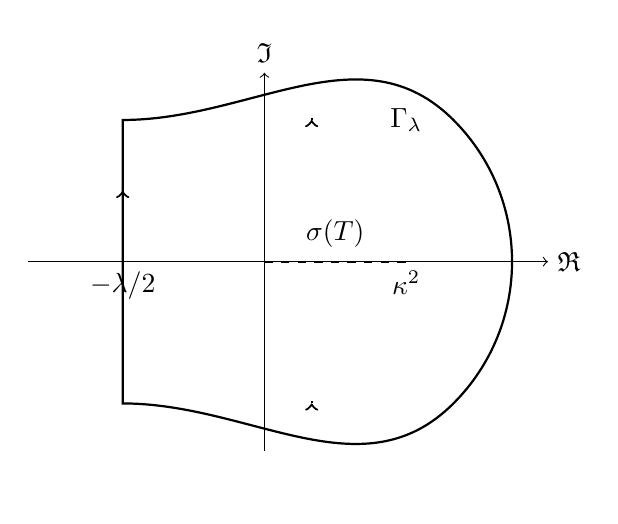
\begin{tikzpicture}[scale=1.2]
    % Coordinate axes
    \draw[->] (-2.5,0) -- (3,0) node[right] {$\mathfrak{R}$};
    \draw[->] (0,-2) -- (0,2) node[above] {$\mathfrak{I}$};
    
    % Contour Γ_λ
    \draw[thick] (-1.5,0) -- (-1.5,1.5) 
        to[out=0,in=135] (2,1.5)
        to[out=-45,in=45] (2,-1.5)
        to[out=225,in=0] (-1.5,-1.5) -- (-1.5,0);
    
    % Spectrum interval
    \draw[dashed, thick] (0,0) -- (1.5,0);
    
    % Points and labels
    \node[below] at (-1.5,0) {$-\lambda/2$};
    \node[below] at (1.5,0) {$\kappa^2$};
    \node at (0.75,0.3) {$\sigma(T)$};
    \node at (1.5,1.5) {$\Gamma_\lambda$};
    
    % Direction arrows on contour
    \draw[->, thick] (-1.5,0.75) -- (-1.5,0.75);
    \draw[->, thick] (0.5,1.5) -- (0.5,1.5);
    \draw[->, thick] (0.5,-1.5) -- (0.5,-1.5);
\end{tikzpicture}

\end{document}